%!TEX root = ../main.tex
%
\section{Ball and plate}
\begin{frame}
	\frametitle{Ball and plate}
\end{frame}
%
\begin{frame}
\frametitle{Ball and plate}
%
\begin{figure}
		{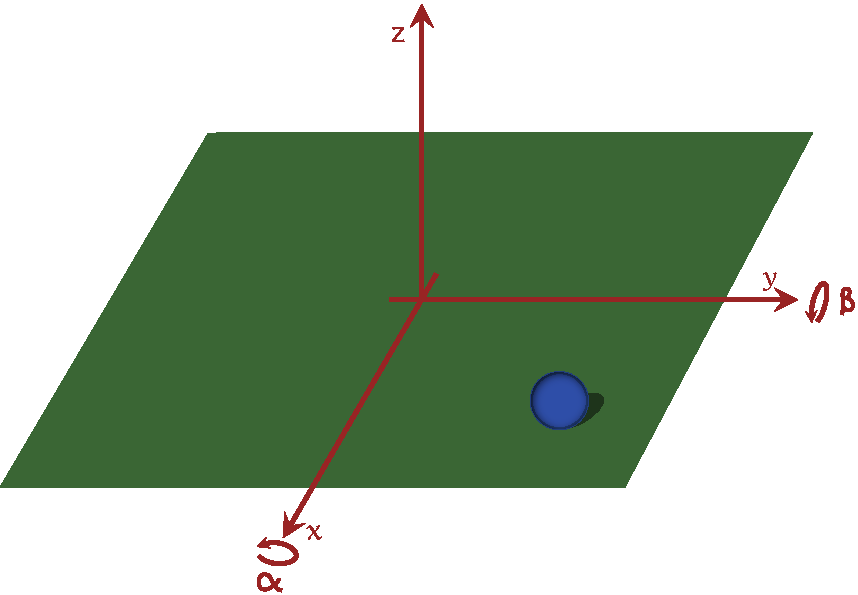
\includegraphics[width=.8\linewidth]{img/ballplate.pdf}}
		\caption{Coordinate frame of the ball and plate system}
		\label{fig:BallPlate}
\end{figure}
\end{frame}
%
\begin{frame}
\frametitle{Ball and plate - Parameters}
\begin{table}
\begin{center}
\begin{tabu} to \textwidth { | X[c] | X[c] | X[c] | }
	\hline
	\textbf{Parameter} & \textbf{Description} & \textbf{Value} \\
	\hline
	$m$ & Mass of the ball & $0.0109 \, Kg$ \\
	$r$ & Radius of the ball & $0.01 \, m$ \\
	$I_b$ & Ball inertia & $4.3563e^{-7} \, Kg\times m^2$ \\
	$l_p$ & Plate side & $0.6 \, m$ \\
	$I_p$ & Plate inertia & $0.175 \, Kg\times m^2$ \\
	\hline
\end{tabu}
\caption{Ball and plate geometric and dynamic parameters}
\label{tab:BallPlate_param}
\end{center}
\end{table}
\end{frame}
%
\subsection{Dynamic}
\begin{frame}
\frametitle{Ball and plate - Dynamic model}
%
The general form of Euler-Lagrange for dynamic equations is used to describe the system:
%
\begin{equation}
	\frac{d}{dt}\frac{\delta T}{\delta q_i} - \frac{\delta T}{\delta q_i} + \frac{\delta V}{\delta q_i} = Q_i
\end{equation}
%
Where $T$ is the kinetic energy, $V$ is the potential energy, $Q_i$ is the i-th generalized force and $q_i$ id the i-th generalized coordinate. As generalized force we consider two torques acting on the plate $(Q_\alpha = \tau_\alpha, Q_\beta = \tau_\beta)$. As generalized coordinates we select two ball position coordinates $[x, y]$ on the frame fixed to the plate and two plate inclination $[\alpha, \beta]$.
\end{frame}
%
\begin{frame}
\frametitle{Ball and plate - Dynamic model}
%
Kinetic energy of the ball:
\begin{equation}
	T_{b} = \frac{1}{2}mv^2 + \frac{1}{2}I_b\omega^2 = \frac{1}{2}\left(m+\frac{I_b}{r^2}\right)\left(\dot{x}^2+\dot{y}^2\right)
\end{equation}
%
Kinetic energy of the plate:
\begin{equation}
	T_{p} = \frac{1}{2}\left(I_b + I_p\right)\left(\dot{\alpha} + \dot{\beta}\right) + \frac{1}{2}m\left(\dot{\alpha}x + \dot{\beta}y\right)^2
\end{equation}
%
Potential energy:
\begin{equation}
	V = mgh = mg(x\,sin\alpha + y\,sin\beta)
\end{equation}
\end{frame}
%
\begin{frame}
\frametitle{Ball and plate - Dynamic model}
%
After some derivations we find the following non-linear system of equations:
%
\begin{align}
	\left(m + \frac{I_b}{r^2}\right)\ddot{x} &- m\left(\dot{\alpha}\dot{\beta}y + \dot{\alpha}^2x\right)+mg\,sin\alpha = 0 \nonumber \\
	\left(m + \frac{I_b}{r^2}\right)\ddot{y} &- m\left(\dot{\alpha}\dot{\beta}x + \dot{\beta}^2y\right)+mg\,sin\beta = 0 \\
	\left(I_p + I_b + mx^2\right)\ddot{\alpha} &+ m\left(\ddot{\beta}xy + \dot{\beta}\left(\dot{x}y + x\dot{y}\right) + 2\dot{\alpha}\dot{x}x\right) +mgx\,cos{\alpha} = \tau_\alpha \nonumber \\
	\left(I_p + I_b + my^2\right)\ddot{\beta} &+ m\left(\ddot{\alpha}xy + \dot{\alpha}\left(\dot{x}y + x\dot{y}\right) + 2\dot{\beta}\dot{y}y\right) +mgy\,cos{\beta} = \tau_\beta \nonumber
\end{align}
\end{frame}
%
\begin{frame}
\frametitle{Ball and plate - Dynamic model}
%
We express the dynamic in matrix form:
%
\begin{equation}
\begin{aligned}
M(q) &=%
\begin{bmatrix}
	\left(m + \frac{I_b}{r^2}\right) &0 &0 &0\\
	0 &\left(m + \frac{I_b}{r^2}\right) &0 &0\\
	0 &0 &\left(I_b + I_p + mx^2\right) &mxy\\
	0 &0 &mxy &\left(I_b + I_p + my^2\right)
\end{bmatrix}\\
C(q,\dot{q}) &=%
\begin{bmatrix}
	0 &0 &-\dot{\alpha} x &-\dot{\alpha} y\\
	0 &0 &-\dot{\beta} x &-\dot{\beta} y\\
	2\dot{\alpha}x &0 &0 &\left(\dot{x}y+x\dot{y}\right)\\
	0 &2\dot{\beta}y &\left(\dot{x}y+x\dot{y}\right) &0
\end{bmatrix}\\
G(q) &=%
\begin{bmatrix}
	mg\,sin\alpha\\
	mg\,sin\beta\\
	mgx\,cos\alpha\\
	mgx\,cos\beta
\end{bmatrix}
\end{aligned}
\end{equation}
%
\end{frame}
